\chapter{Measurement technique}
\section{Heating}
\label{sec:heating}
This section will be devoted to the following topics:
\begin{enumerate}
	\item The circuit design to achieve mK level broadening in the thermal reservoir while preventing any potential from developing in the reservoir, which would effectively shift the chemical potential of the reservoir.
	\item Techniques used to apply synchronously apply two, 90$^{\circ}$ out of phase square wave heating signals on either side of a remote quantum point contact, allowing for heating in separate bath while preventing a monopole electric moment from affecting the entropy measurement.
\end{enumerate}

\section{Extraction of dN/dT signal}
\label{sec:data_analysis}
This section will be devoted to the following topics:
\begin{enumerate}
	\item The techniques used to allow for repeated measurements and used to fit and extract entropy signals.
\end{enumerate}


\section{Artifacts from cross couplings}
\label{sec:artifacts}
The focus of this section will be explanations of the artifacts that are notably present in dN/dT data presented in this thesis. See 



\section{Determination of electron temperature}
This section will focus on methods for determination of electron temperature in this system as well as the methodology we have employed to achieve these temperatures. With specific reference to Fig. \ref{fig:etemp}.

\label{sec:electrontemp}
\begin{figure}[h]
\centering
\resizebox{1\textwidth}{!}{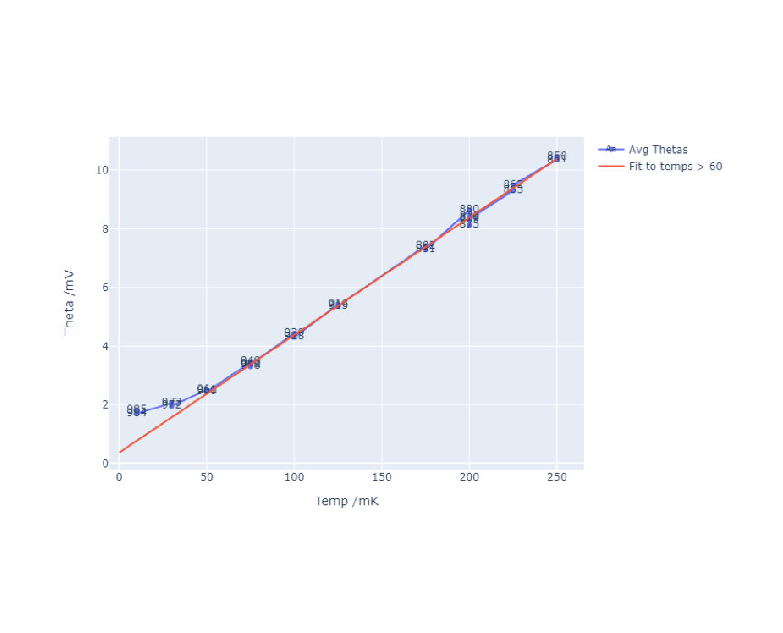
\includegraphics{figures/pdfs/temp_electron_temp.eps}}
\caption{By fitting the transition line shapes of the 0 $\to$ 1 electron transition in the quantum dot, one can extract the broadening of the fermi energy in the reservoir. By varying the lattice temperature of the substrate and plotting the effective broadening of the fermi sea ($\theta$) at each lattice temperature, we can extract the effective electron temperature, $T_e$. Here $T_e \approx 35$ mK. }

\label{fig:etemp}       % Give a unique label to the figure. 
\end{figure}

\chapter{Measurement setup}
This section will include 
\begin{itemize}
\item Detailed description of experimental techniques by which data are collected
\item Samples of multiple levels of data through processing
\end{itemize}

\chapter{Device Fabrication}
This section will include 
\begin{itemize}
\item Processes which are followed for the production of devices on a GaAs substrate
\item Various check lists for processes (space depending).
\end{itemize}
